%\addcontentsline{toc}{chapter}{Development Process}
\chapter{Design}

% You should concentrate on the more important aspects of the design. It is essential that an overview is presented before going into detail. As well as describing the design adopted it must also explain what other designs were considered and why they were rejected.

% The design should describe what you expected to do, and might also explain areas that you had to revise after some investigation.

% Typically, for an object-oriented design, the discussion will focus on the choice of objects and classes and the allocation of methods to classes. The use made of reusable components should be described and their source referenced. Particularly important decisions concerning data structures usually affect the architecture of a system and so should be described here.

% How much material you include on detailed design and implementation will depend very much on the nature of the project. It should not be padded out. Think about the significant aspects of your system. For example, describe the design of the user interface if it is a critical aspect of your system, or provide detail about methods and data structures that are not trivial. Do not spend time on long lists of trivial items and repetitive descriptions. If in doubt about what is appropriate, speak to your supervisor.
 
% You should also identify any support tools that you used. You should discuss your choice of implementation tools - programming language, compilers, database management system, program development environment, etc.

% Some example sub-sections may be as follows, but the specific sections are for you to define. 

\section{Overall Architecture}
The design of my application was evolutionary as I was developing it using XP in an agile way. This meant that each step had an initial design and was built upon every time a new feature was added, being refactored along the way. There were a number of prototypes made during the course of the project's development, and this chapter will discuss the design of the end product, and go into detail where the design may have been previously different.

The resulting application evolved into a web service, with a Model View Controller (MVC) framework and resources structured for maintainability. Following XPs guidelines, at each step of the way the applications design was made as such to be the simplest yet most maintainable it could be through refactoring, cutting down on duplicate code, structured logically and choosing smart data structures and Objects to represent aspects of the application and quality results.

\subsection{Choice of technologies}
At the beginning of the application, I felt that the application should be programmed in a language that would be able to be ported across multiple platforms for used by anybody who wished to use it. Additionally to this, I wanted to have ways of representing the components of my application as Objects and would need some way of presenting a UI to the user, even if my initial application would only output command line results, in order to follow the XP value of Simplicity (YAGNI - ``You Ain't Gonna Need It'', until you do).

For this reason, I selected to develop my application using Java to begin with as it filled the criteria of being Object Oriented and was portable through using the JVM on different operating systems. I resolved that I would select a UI package to present the report of my results once some of the core functionality had been implemented. I considered instead using Ruby or C++, but due to my familiarity with Java I believed it would be a better choice to stick with what I knew. At this point, I did not consider having the application as a web service, and so using Ruby with Rails was not something I had considered.

As the application developed and I started reading in files and outputting results from the GC Content process, I found that I was having a hard time finding a quickly usable GUI I could work with for Java to display the results in a way that I wanted. It was at this point I started considering a technology change to Ruby on Rails until Sion Griffiths, a peer of mine, suggested I could keep my application in Java and turn it into a web service using Spring Boot\cite{springboot}. This seemed like the perfect solution to my problem, allowing me to generate my charts and results using HTML5, JavaScript and HTML5 Canvas, along with JavaScript libraries such as  Plotly.js.

The conversion to Java Spring Boot was not a painful one, and only involved setting up a new Maven project and declaring it to run as a Spring Boot application in the pom.xml file, then copying over my previous code and structure into the new project, from there I could deploy the application as a web server using Tomcat and was back to my previous position of working out a UI. Thankfully, there is a package called Thymeleaf\cite{thymeleaf} that works with Spring Boot to allow access to Objects from within the Model of the Java code (placed there by the Controller) using the View dynamically as the View is generated through HTML templates and fragments.

\begin{figure}[H]
	\centering
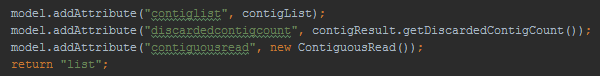
\includegraphics[width=1\textwidth]{images/addingtomodel}
\caption{Adding an object to the Model via the Controller to be accessed in the View. The View here is `list', which is a Thymeleaf template that will dynamically build the page using the data from the Model added here.}
\end{figure}

On top of using Thymeleaf for accessing data put into the Model, it has the additional benefit of using fragments that can be imported into different HTML templates. This design choice made it so I was able to cut down on writing duplicates of code. For example, I wrote the header and footer of the UI design in a Thymeleaf HTML fragment, and then on each page just need to call one line in order to import it into that page, rather than built the entire thing again. An extra benefit to this is that it allowed me to keep the HTML templates clean and easier to maintain by reducing their size and separating out different aspects of the UI. Having the header, footer and a number of forms in Thymeleaf HTML templates meant that these sections could be edited without impacting any page they are imported into.

\begin{figure}[H]
	\centering
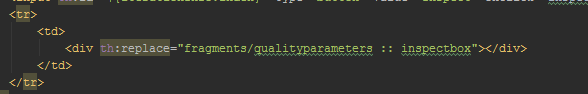
\includegraphics[width=1\textwidth]{images/thymeleafinsert1}
\caption{Including a thymeleaf fragment in a page. You can see how the call is made from one `th:replace' with the name of the html fragment file and then the fragment to be included from that file, in this case `inspectbox'.}
\end{figure}
\begin{figure}[H]
\centering
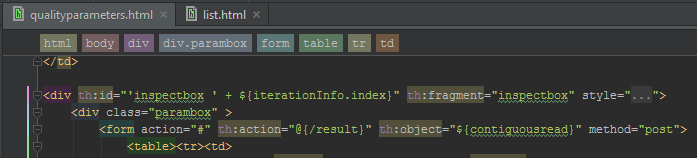
\includegraphics[width=1\textwidth]{images/thymeleafinsert2}
\caption{Including a thymeleaf fragment in a page. This is the declaration of the fragment being included in the previous figure, declared as such through `th:fragment'.}
\end{figure}

For the GUI itself, I elected to use Plotly for representing my GC content charts for the level of detail and control it gives a user over inspecting charts, large and small, that worked no matter what GC window size the user selected. For the ORF Locations frames charts I wrote my own code using JavaScript and displayed it with HTML5 Canvas, as it allowed me control over what should be shown depending what a user clicks upon and I could work with the data from the Model in ways I saw fit.

%=== Up to here

Started by considering what langauge would be appropriate for the processing and display, and at first thought Java would be a good idea. Lead on later to realizing I wanted more than just what Java could do by itself, and chose to make a web serivice, using Java Spring Boot, deployed with Tomcat. I could have instead at this point switched to using Ruby on Rails, but with my prototype code for the GC Content percentage finder done in Java, and without the need for any Active Record, it felt like Java would be the better option. Also portable, as the data processed may be quite large, so Java to allow the application to be run through the JVM on any system (e.g. a Linux HPC) would be appropriate.
Why Java instead of Ruby, for example?
Why use Javascript once I decided to use a web service. Because of Plotly and Canvas? Usability? Accessing data. How about how the data is structured in Javascript?
Why did I select plotly and canvas in particular? Fine level control in canvas, ease of use with Plotly, allowing a user far greater control over viewing their charts than I could provide in the time.
Why thymeleaf? very useful for accessing Object data provided by the model. Using fragments for importing sections - Helps remove duplicate code, e.g. for importing the header, and keeping files clean and changing internals of particular charts in their own files, e.g. qualityparameters.html fragment.


\subsection{MVC Framework}
\subsubsection{Model}
Data and structure. ORF sections, GC sections, utility classes and functions, controller access
\subsubsection{View}
Building the view with Javascript and HTML5, using thymeleaf to access data in an OO way.
Choice of designing for the view, let it have the data from the Model, passed from the Controller, and how it deals with displaying the data is completely down to the view. Could develop some parts of the view within the code and pass that to the View, but decided it would be better to instead pass the data as is, and let the view decide on the way of display. This allows the front-end and design of the view to be changed in the future without having to go into the internals of the code base and Model itself to change. Keeping the View and Model separate.
\subsubsection{Controller}
Access through GET and POST methods, validation through Java Spring, response to requests and putting objects into the model to be accessed via thymeleaf, through the controller and put into the view. 

RESTful interface? GET/POST with session parameters. URL is basic 'list' 'toolkit' 'welcome' represents what you get and addressable when needed. (Remind yourself about the principles of REST and talk about them here!!).

\subsection{Object Oriented and Method Naming}
OO approach relevant to represent things as Objects. Such as a GC result, ORF Result, etc. Easy to access these items in the browser through thyemleaf as Objects with known names and properties.

Method names follow the convention likeThisSortOfThing and will also try to explain what they do in the method name. Likewise, variables and fields are named such that you can understand what they are without commenting. Attempting to make code that reads for itself what it is. Have JavaDoc for all classes to clarify anything that isn't easily understandable from the code itself.

\subsubsection{User Input}
FASTA file format - Standard format for assembly data.
Considered File Uploads, and still contains the code for doing this, used for my test files, however, pasting user content was more secure and acceptable for testing. The code for file uploads still exists to be used in revisions to the application.
Data is processed in a FASTA reader, and does these things...
This way of handling the data, returning it to the controller, and then passing it on to the toolkit area of the model to be 'qualityAssessed', where there are the calls to the techniques used. Again, in a future revision and with more techniques, it may be worth while to allow the user to disable or enable particular techniques they are interested in.

User data is not kept by the application, it is stored in a user session that expires once they leave the page. This is handled by Java Spring, and set as a @sessionvariable (..), show an example image of these in the code. If the user does not have their session variables, they are presented with the Error page, so they cannot try and access areas of the application/web service where they currently do not have access or the data to do so.

\subsection{Directory Structure}
Java Code stored in three sections. Main is top level, going down into Domain code, Utility code and Web code. All resources, such as stylesheets, html files and javascript stored under resources folder in static directory. HTML stored as template .html files for use by Thymeleaf, Javascript broken up into multiple files based on where they are used (toolkit.js, list.js) and their functions (orf-chart.js, gc-chart.js). Separating out the files this way improves readability and maintainability. Keeping things isolated and simple.

Using MVC - What is MVC - What else did I consider? Did I think about using a command line tool, why no good? Report output. What about using something not a web service? Why did I choose to do a web service instead?

Started working on Java code with the intention of making a GUI that would do the things. Decided


\subsection{QualitySummary}
Results returned in a QualitySummary object. Object contains references to GcResult and OpenReadingFrameResult. Option to have these two implement an interface that might be called QualityResults, and have just an array of QualityResults. This would allow us to add any type of result without needing to know what is in there. However, chose not to do this as considering the way in which we serve the view results and them being so tightly coupled to the view, didn't seem necessary through the evolutionary design. Aware that in the future if we allowed a user to select what type of processing they wish to use, this technique would be very useful to implement, and only serve up the results tabs that they wish to see. However, as stated, evolutionary design through TDD so wasn't yet necessary.

Show how the design is structured. How do we go from the file to the processing? Why did I do it this way? What were my initial designs.
Considering ORFS - Result is an ArrayList of the OpenReadingFrameLocations, why this way? First looking at just 'the longest', then prototyping it out to find one in each frame, then breaking it out into finding Start/Stop Codons and 'stitiching' them together where appropriate.

\section{User Interface}
Framework mock ups of the user interface. Logo for kicks.

- Input form, why is it this way?
- List - Displaying each contig, why, framework, drop downs
- Paramters - Why did I pick these Paramters, what use are these for the user? Why GC content windows and what size is reasonable? Can demonstrate domain knowledge about the choice of parameters. Up to the user, allowing them to put in stupid numbers, but their results are their own.
- GC Chart - Why does it look like this - Choice of standard deviation and mean, why? What use does this actually have  in showing the user error areas? What about just visually seeing the data? Show the screenshots of areas out of GC content threshold, show the areas where obvious chimera (50/50 example)
- ORF Location - Why did I develop it to look like this? Representing each of the 6 frames, demonstrate the reverse frames are displayed in the correct direction. How did I achieve this and why display it this way and the inner detail? Other approaches? What about the NCBIs version? Ability to click. Also the list? Why have both? They're both useful to have, as a user may want to look at the shortest ORF Location but not be sure where it is even when they read what frame it is. Likewise they may want to see where an ORF Location lies in the list organized into longest to shortest. Why organized into length. Useful to the user to get an idea to further inspect. Why 6 different canvases for the frames? Easier to modify and display on the page.
- Superframe - What is it and why did I consider it. Showing overlaps and where the Red areas may be areas of errors and what to look for. The explanation of it, why explain it this way? 

\section{Support Tools}
For writing the code, I used JetBrains IntelliJ IDE (screenshot of IDE window with some code). This included writing all the code, Java, HTML, CSS, Javascript, ThymeLeaf and any additional properties for setting up Spring Boot. Useful for text highlighting, debugging the code, and tied into my version control, using Git and hosted on GitHub. (screenshot of commits)
\subsection{Version Control}
Using version control to keep a repository of code in case of lost data in event of hardware crash or software corruption. GitHub decent choice, already had a repository on there and Git supported in IntelliJ IDE. In addition, every time I check in, I used continuous integration with CodeShip, allowing me to receive e-mails any time I made a commit to my repo that didn't pass the tests written. Very helpful in discovering issues with failing builds when checking in a change and forgetting to update tests or breaking previously written code as the design changed (show screenshot of failing/passing builds from CodeShip).